\chapter{الخلايا الجذعية، والتجدد، والشيخوخة}\label{ch:b3:stem-cells}

اقطع رجل أكسولوتل تجده في شهرين قد أنمى رجلًا جديدة، عظمًا
وعضلًا وعصبًا وجلدًا في مواضعها الصحيحة، وسيفعل ذلك كلما
قطعت. واقطع دودة مفلطحة من البلاناريا عشرين قطعة تجد كل قطعة
تصير دودة كاملة في أسبوعين، والقطعة التي كانت ذنبًا تُنمي
رأسًا بعينين ودماغ. واقطع إصبع إنسان فوق المفصل الأخير يلتئم
ندبةً. ومع ذلك فجسم الإنسان ليس بلا \omterm{def:b3:stem-cells:regeneration}{تجدد}: ففي كل ثانية يصنع
مليوني كرية دم حمراء، وتُستبدل بطانة الأمعاء كل خمسة أيام،
والجلد كل شهر، وكل ذلك منحدر من جمهرات صغيرة من الخلايا
تنقسم طوال العمر بلا أن تستنفد نفسها. وهذا الفصل عن تلك
الخلايا --- ما الذي يجعل \omterm{def:b3:stem-cells:stem}{الخلية جذعية}، وكيف تحفظها حاضنتها،
وكيف يُبنى منها تراتب الدم أو الأمعاء كله --- وعن الحيوانات
التي تقدر على إعادة إنماء ما لا نقدر عليه ولماذا، وعن اكتشاف
أن أي خلية يمكن دفعها راجعةً إلى الحالة الجنينية بأربع
مورّثات، وعمّا يقوله حساب انقسام الخلايا في سبب شيخوختنا.

\section{ما الخلية الجذعية}

\begin{definition}[الخلايا الجذعية وتراتبها]\label{def:b3:stem-cells:stem}
\index{خلية جذعية}\index{تجدد ذاتي}\index{انقسام لامتناظر}\index{سليفة}\index{خلية عبور مضخِّمة}\index{حاضنة}
\emph{للخلية الجذعية} خاصتان تعرّفانها: أنها تقدر على
\emph{\omterm{def:b3:stem-cells:regeneration}{التجدد} الذاتي}، فتنتج بنات هنّ خلايا جذعية، وأنها تقدر
على إنتاج بنات يتمايزن. وقد تفعل الأمرين معًا،
\emph{بانقسام لامتناظر}، بنتًا من كل صنف، ويحدد المصير
توريثٌ غير متساوٍ للمحدِّدات أو أيّ البنتين تبقى على تماس
\emph{الحاضنة} --- أي البيئة الدقيقة من الخلايا المجاورة
والمهد والإشارات التي تُبقي الخلية جذعية؛ أو قد تنقسم
انقسامًا متناظرًا، فتعطي بعض الانقسامات خليتين جذعيتين
وأخرى خليتين متمايزتين، مع بقاء الجمهرة ثابتة في المتوسط.
والبنات المتمايزات يمررن عادةً بمراحل \emph{سليفة} أو
\emph{عبور مضخِّمة}، فينقسمن عدة مرات أخرى بقدرة تضيق قبل أن
ينضجن: فالتراتب يضخّم انقسامات جذعية بطيئة قليلة إلى خرج
كبير، ويحدّ عدد الانقسامات التي على أي خلية جذعية أن تقوم
بها. والخلايا الجذعية البالغة نادرة بطيئة --- فالخلية
الجذعية المكوِّنة للدم تنقسم مرة في السنة لعلّ، والخلية
الجذعية المعوية مرة في اليوم --- وهي \emph{متعددة القدرات}،
محصورة في سلالات نسيجها؛ وأما الخلايا الجذعية الجنينية، من
كتلة الخلايا الداخلية في الكييسة الأرومية، فهي \emph{كاملة
القدرات}، قادرة على صنع كل نسيج في الجسم لا المشيمة.
\end{definition}

\begin{omfigure}
\begin{tikzpicture}[every node/.style={font=\scriptsize}, >=stealth]
  \node[draw, very thick, rounded corners, fill=omDef!25, align=center] (hsc) at (0,3.6) {خلية جذعية مكوِّنة للدم\\$\sim$\num{10000} في الإنسان؛ وتنقسم $\sim$ مرة في السنة};
  \node[draw, thick, rounded corners, fill=omDef!12, align=center] (mpp) at (0,2.4) {سلائف متعددة القدرات};
  \node[draw, thick, rounded corners, fill=omThm!15, align=center] (cmp) at (-3.2,1.2) {سليفة نقوية};
  \node[draw, thick, rounded corners, fill=omProp!20, align=center] (clp) at (3.2,1.2) {سليفة لمفية};
  \node[align=center, font=\tiny] (e) at (-5.4,-0.4) {كريات حمر\\$2\times 10^{11}$/يوم};
  \node[align=center, font=\tiny] (pl) at (-3.6,-0.4) {صفيحات\\(نويّات ضخمة)};
  \node[align=center, font=\tiny] (g) at (-1.8,-0.4) {محببات\\$10^{11}$/يوم};
  \node[align=center, font=\tiny] (m) at (-0.2,-0.4) {وحيدات النواة،\\والبلعميات};
  \node[align=center, font=\tiny] (b) at (1.8,-0.4) {لمفاويات بائية};
  \node[align=center, font=\tiny] (t) at (3.4,-0.4) {لمفاويات تائية};
  \node[align=center, font=\tiny] (nk) at (5.0,-0.4) {خلايا قاتلة طبيعية};
  \draw[->, thick] (hsc) -- (mpp); \draw[->, thick] (mpp) -- (cmp); \draw[->, thick] (mpp) -- (clp);
  \foreach \x in {e,pl,g,m} { \draw[->, thick] (cmp) -- (\x); }
  \foreach \x in {b,t,nk} { \draw[->, thick] (clp) -- (\x); }
  \draw[->, thick, omDef!70!black] (hsc.west) .. controls (-3.0,4.4) and (-3.0,3.0) .. (hsc.south west) node[pos=0.5, left, font=\tiny, omDef!70!black, align=right] {تجدد ذاتي};
  \node[right, align=left, font=\tiny] at (4.4,3.6) {كل طبقة تنقسم أكثر\\وقدرتها أضيق؛\\و$\sim 20$ انقسامًا من الخلية الجذعية\\إلى الكرية الحمراء، فانقسام واحد\\لخلية جذعية يعطي $\sim 10^{6}$ خلية};
\end{tikzpicture}

{\small تراتب تكوين الدم. بضعة آلاف من الخلايا الجذعية
البطيئة في النقي تغذي سلائف تنقسم سريعًا وتلتزم تدريجًا،
فيكلف خرجٌ من تريليون خلية في اليوم الخلايا الجذعية ما لا
يكاد يُذكر.}
\end{omfigure}

\begin{proof}[شواهد]
حقن تِل ومكولوك (1961) خلايا نقي في فئران مشععة تشعيعًا
قاتلًا وعدّا العقيدات التي ظهرت على الطحال بعد عشرة أيام:
فكانت كل واحدة مستعمرة من خلايا دم من سلالات عدة، وعددها
متناسب مع الخلايا المحقونة، وأظهر وسم صبغيات خلايا المتبرع
أن كل مستعمرة نسيلة --- أي إن خلية واحدة صنعت كريات حمرًا
ومحببات وصفيحات، وحوت بعض المستعمرات خلايا تقدر على بذر
مستعمرات جديدة في فأر ثانٍ: أي \omterm{def:b3:stem-cells:stem}{تجدد ذاتي} وتعدد قدرات في
خلية واحدة، وهو التعريف الإجرائي \omterm{def:b3:stem-cells:stem}{للخلية الجذعية}، وأساس زرع
نقي العظم. ووسم باركر وكليفرز (2007) الخلايا المعبِّرة عن
المورّثة \emph{Lgr5} في قاعدة الخبيئات المعوية بلون موروث
وراقبا، على مدى أسابيع، اللون يتسلق الخبيئة ويملأ زغابات
كاملة: فالخلايا الموسومة كانت الخلايا الجذعية للأمعاء،
وواحدة منها، مستنبتة في هلام بعوامل النمو الثلاثة الصحيحة،
نمت إلى أمعاء مصغَّرة، أي \emph{\omterm{def:b3:stem-cells:pluripotency}{عُضْوانية}}، لها خبيئاتها
وزغاباتها (ساتو، 2009).
\end{proof}

\begin{proposition}[الحاضنة والخبيئة]\label{prop:b3:stem-cells:crypt}
\index{خبيئة}\index{Lgr5}\index{خلية بانيث}\index{إشارة Wnt}\index{انجراف محايد}
\emph{الخبيئة} المعوية أفضل الحاضنات فهمًا. ففي قاعدتها نحو
أربع عشرة \omterm{def:b3:stem-cells:stem}{خلية جذعية} \emph{Lgr5} محشورة بين خلايا بانيث،
التي تفرز إشارتي Wnt وNotch وعوامل النمو التي تبقيها خلايا
جذعية؛ \omterm{def:b3:stem-cells:stem}{والخلية الجذعية} التي تُدفع إلى أعلى خارج تماس خلايا
بانيث تفقد الإشارة في غضون بضعة أقطار خلوية وتصير \omterm{def:b3:stem-cells:stem}{خلية عبور
مضخِّمة}، تنقسم أربع مرات أو خمسًا في الخبيئة ثم تتمايز إلى
الخلايا الامتصاصية والإفرازية التي تهاجر إلى أعلى الزغابة
وتُنبذ من طرفها بعد خمسة أيام. وتنقسم الخلايا الجذعية
انقسامًا متناظرًا، نحو مرة في اليوم، وتتنافس على حيّز
\omterm{def:b3:stem-cells:stem}{الحاضنة} المحدود: فتتوسع نسيلة واحدة بالمصادفة وتضيع الأخريات،
حتى تصير كل خبيئة في غضون أشهر قليلة منحدرة من \omterm{def:b3:stem-cells:stem}{خلية جذعية}
واحدة --- أي \emph{\omterm{prop:b3:stem-cells:crypt}{انجراف محايد}} على مقياس خبيئة، مشيًا
عشوائيًا بحدود ماصّة. \omterm{def:b3:stem-cells:stem}{والحاضنة}، لا الخلية، هي التي تحفظ
الجذعية: فأعِد خلية متمايزة إلى تماس إشارات بانيث بعد أذية
تقدر على الارتداد؛ وأخرِج \omterm{def:b3:stem-cells:stem}{الخلية الجذعية} وأعطها الإشارات في
طبق تصنع \omterm{def:b3:stem-cells:pluripotency}{عُضْوانية}. ونقي العظم، وجريبات الشعر، والخصية،
ومناطق الخلايا الجذعية العصبية في الدماغ تتبع المنطق نفسه
بإشارات مختلفة.
\end{proposition}
\begin{proof}[شواهد]
وسم سنيبرت وزملاؤه (2010) الخلايا الجذعية في الخبيئات
بألوان ``كونفيتّي'' أربعة عشوائية؛ فكانت الخبيئات متعددة
الألوان في البداية وصارت أحادية اللون في غضون أشهر قليلة،
بمعدل يطابق الانقسام المتناظر والتنافس المحايد بين نحو أربع
عشرة خلية --- لا \omterm{def:b3:stem-cells:stem}{الانقسام اللامتناظر}، الذي كان سيبقي كل لون
إلى ما لا نهاية. وإزالة خلايا بانيث تقلّص مجمع الخلايا
الجذعية؛ وإزالة \omterm{prop:b3:stem-cells:crypt}{إشارة Wnt} تفرغ الخبيئة في أيام.
\end{proof}

\begin{omfigure}
\begin{tikzpicture}[every node/.style={font=\scriptsize}, >=stealth]
  % crypt-villus
  \draw[very thick, omDef] (0,-2.6) .. controls (0,-0.4) and (0.4,0) .. (0.8,0) -- (0.8,3.6) .. controls (0.8,4.1) and (1.6,4.1) .. (1.6,3.6) -- (1.6,0) .. controls (2.0,0) and (2.4,-0.4) .. (2.4,-2.6);
  \draw[very thick, omDef] (0,-2.6) arc[start angle=180, end angle=360, radius=1.2];
  % stem cells at base
  \foreach \a in {200,230,260,290,320} { \fill[omThm!60] ({1.2+1.05*cos(\a)},{-2.6+1.05*sin(\a)}) circle (0.14); }
  \foreach \a in {215,245,275,305} { \fill[omMeth!60] ({1.2+0.75*cos(\a)},{-2.6+0.75*sin(\a)}) circle (0.13); }
  \node[right, align=left, font=\tiny] at (2.6,-3.4) {القاعدة: $\sim 14$ خلية جذعية \emph{Lgr5} (بالأحمر)\\محشورة بين خلايا بانيث (بالأخضر)،\\التي توفر Wnt وNotch وEGF};
  % TA zone
  \foreach \y in {-1.8,-1.3,-0.8,-0.3} { \fill[omProp!50] (0.35,\y) circle (0.11); \fill[omProp!50] (2.05,\y) circle (0.11); }
  \node[right, align=left, font=\tiny] at (2.6,-1.1) {منطقة العبور المضخِّمة:\\4--5 انقسامات، واحد في اليوم،\\خارج إشارات بانيث};
  % villus cells
  \foreach \y in {0.4,1.0,1.6,2.2,2.8} { \fill[omDef!40] (0.95,\y) circle (0.1); \fill[omDef!40] (1.45,\y) circle (0.1); }
  \node[right, align=left, font=\tiny] at (2.6,1.8) {الزغابة: خلايا متمايزة\\تهاجر إلى أعلى وتُنبذ\\من الطرف بعد $\sim 5$ أيام};
  \node[left, font=\tiny] at (-0.1,-2.6) {خبيئة}; \node[left, font=\tiny] at (0.7,3.9) {طرف الزغابة};
  % confetti panel
  \begin{scope}[shift={(8.8,0.2)}]
    \node[above, align=center] at (0,1.3) {انجراف محايد في الحاضنة};
    \foreach \i/\cols in {0/{omDef!60,omThm!60,omMeth!60,omProp!60,omDef!60,omThm!60}, 1/{omDef!60,omDef!60,omThm!60,omThm!60,omThm!60,omProp!60}, 2/{omThm!60,omThm!60,omThm!60,omThm!60,omDef!60,omThm!60}, 3/{omThm!60,omThm!60,omThm!60,omThm!60,omThm!60,omThm!60}} {
      \foreach [count=\j] \c in \cols { \fill[\c] ({\j*0.36-1.26},{1.0-\i*0.7}) circle (0.15); }
    }
    \node[left, font=\tiny] at (-1.35,1.0) {الأسبوع 0}; \node[left, font=\tiny] at (-1.35,0.3) {الأسبوع 4}; \node[left, font=\tiny] at (-1.35,-0.4) {الأسبوع 12}; \node[left, font=\tiny] at (-1.35,-1.1) {أشهر};
    \node[below, align=center, font=\tiny] at (0,-1.75) {تتنافس النسائل على عدد ثابت\\من الأماكن؛ وتفوز واحدة بالمصادفة};
  \end{scope}
\end{tikzpicture}

{\small الخبيئة حاضنةً. الجذعية موضع: فالخلايا الملامسة
لإشارات خلايا بانيث تبقى جذعية، والخلايا المدفوعة خارج التماس
تبدأ رحلة الأيام الخمسة إلى طرف الزغابة. وإذا وُسمت بألوان
عشوائية، انجرفت خلايا الخبيئة الجذعية إلى نسيلة واحدة في غضون أشهر.}
\end{omfigure}

\section{كمال القدرة وإعادة البرمجة}

\begin{definition}[جنينية، ومحرَّضة، ومستنبتة]\label{def:b3:stem-cells:pluripotency}
\index{خلية جذعية جنينية}\index{كمال القدرة}\index{خلية جذعية كاملة القدرات محرَّضة}\index{إعادة البرمجة}\index{عُضْوانية}
\emph{الخلايا الجذعية الجنينية} (إيفانز، وكوفمان، ومارتن،
1981، في الفأر؛ وطومسون، 1998، في الإنسان) خلايا من كتلة
الخلايا الداخلية تُبقى منقسمة في الاستنبات بلا تمايز،
بإشارات (LIF، أو FGF والأكتيفين) تصون لبًّا من عوامل
الاستنساخ --- Oct4، وSox2، وNanog ---
تفعّل بعضها بعضًا وتكبت مورّثات كل سلالة. وإذا حُقنت في
كييسة أرومية انضمت إلى الجنين وأسهمت في كل نسجه، بما فيها
السلالة الجنسية، وبذلك يُصنع فأر الحذف: غيّر مورّثة في
الخلايا، ثم اصنع منها فأرًا. وقد أظهر النقل النووي في مجلد
السنة الثانية أن نواة متمايزة يمكن أن تُعاد ضبطها بعصارة
البيضة؛ ووجد تاكاهاشي ويامانكا (2006) ما يقوم بإعادة الضبط.
فمن أربع وعشرين مورّثة مرشَّحة، حوّلت أربع --- \emph{Oct4}،
و\emph{Sox2}، و\emph{Klf4}، و\emph{c-Myc} --- أُدخلت معًا على
فيروسات إلى أرومات ليفية جلدية، نحو خلية واحدة من كل ألف
على مدى ثلاثة أسابيع إلى \emph{\omterm{def:b3:stem-cells:stem}{خلية جذعية} كاملة القدرات
محرَّضة} لا تُميَّز عن الجنينية، قادرة على تكوين كل نسيج
وعلى تكوين فأر كامل. و\emph{إعادة البرمجة} بطيئة قليلة
النجاعة لأن على العوامل أن تفتح صبغينًا أغلقته سنوات من
التمايز، ولأن الخلايا تمر بطور عشوائي يتعثر فيه معظمها؛ وهي
أيضًا، من حيث المبدأ، طريق من خلايا المريض نفسه إلى أي نسيج.
وأضِف الإشارات الصحيحة بالترتيب الصحيح تُعِد الخلايا الكاملة
القدرات في طبق سردَ النماء: عضلة قلب تنبض، وعصبونات دوبامينية
للزرع في دماغ باركنسوني، وخلايا \omterm{def:b3:sensory-systems:retina}{شبكية}، و\emph{عُضْوانيات}
--- نسج ثلاثية الأبعاد ذاتية التنظيم عرضها بضعة ميليمترات،
معوية وكلوية وكبدية ومخية، بمعمار العضو وأنماط خلاياه، يمكن
أن يُراقَب فيها نماء الإنسان ومرضه وأن تُختبر الأدوية.
\end{definition}

\begin{omfigure}
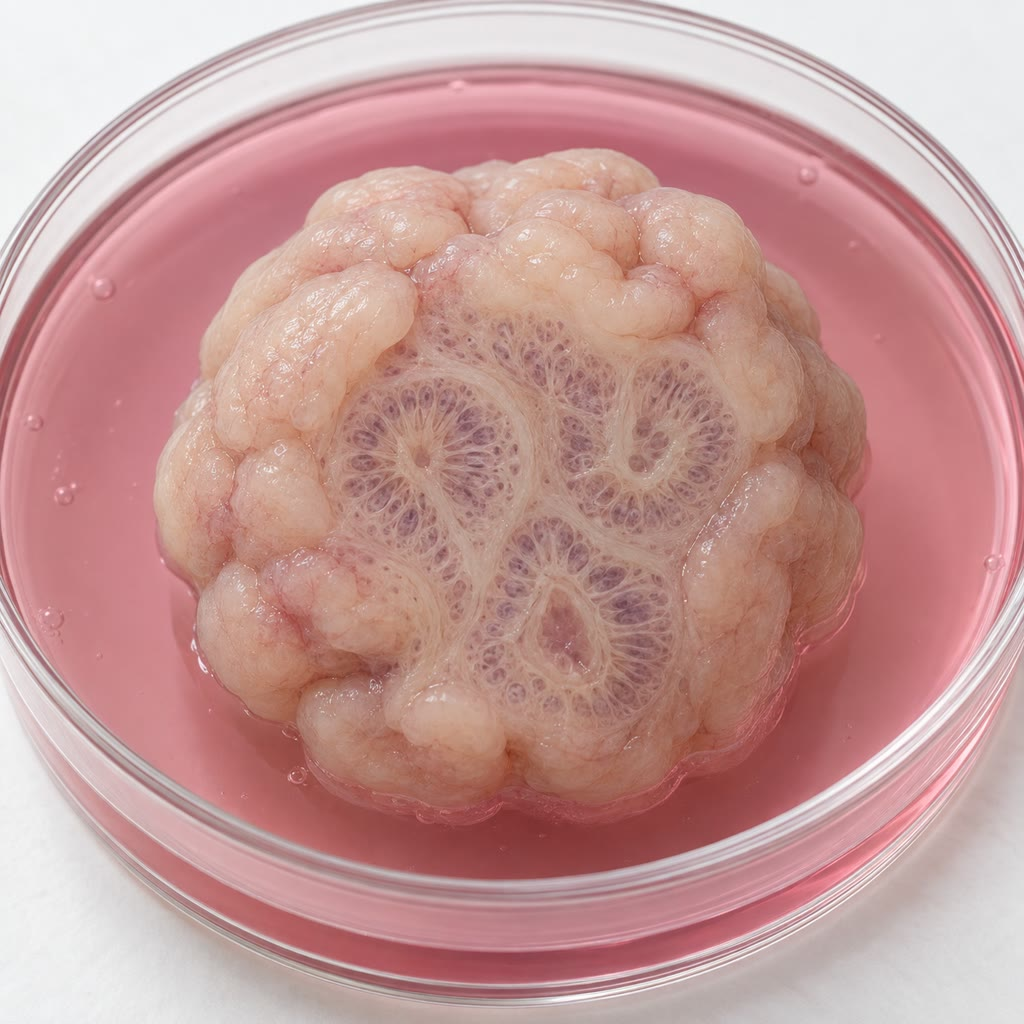
\includegraphics[width=0.4\linewidth]{images/book5/ai/b5-24-brain-organoid.jpg}\hspace{0.04\linewidth}
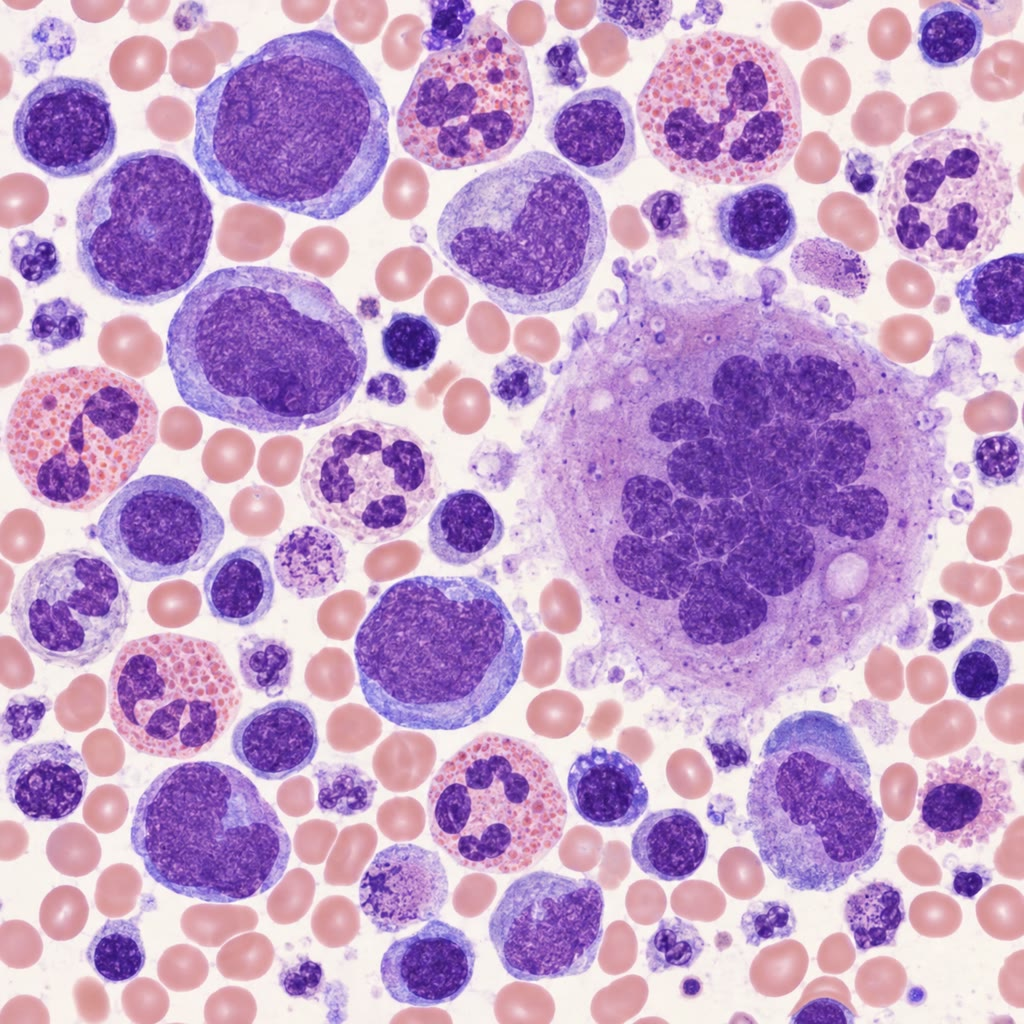
\includegraphics[width=0.4\linewidth]{images/book5/ai/b5-24-bone-marrow-smear.jpg}

{\small يسارًا: \omterm{def:b3:stem-cells:pluripotency}{عُضْوانية} مخية نمت من خلايا بشرية كاملة
القدرات --- بضعة ميليمترات من نسيج شبيه بالقشرة ذاتي التنظيم،
بتجاويف شبيهة بالبُطينات وعصبونات مطبَّقة. ويمينًا: لطاخة
نقي عظم، وفيها تراتب الشكل الأول مرئيًا دفعةً واحدة:
أرومات، ومحببات ناضجة، وسلائف كريات حمر، ونويّة ضخمة.}
\end{omfigure}

\begin{method}[تتبع السلالة]\label{met:b3:stem-cells:tracing}
\index{تتبع السلالة}\index{ريكومبيناز Cre}
لمعرفة أي الخلايا هي الخلايا الجذعية لنسيج: (1) اختر مورّثة
تعبّر عنها الخلايا المرشَّحة وضع تحت مروّجها ريكومبيناز
قابلًا للاستحثاث (Cre-ER، لا يكون فعالًا إلا حين يُعطى
التاموكسيفين)؛ (2) وفي الحيوان نفسه، مورّثة كاشفة تصير فعالة
على الدوام حين يقطع الريكومبيناز منها كاسيت وقف --- أي لونًا
يرثه كل خلف؛ (3) أعطِ جرعة واحدة من التاموكسيفين لوسم
الخلايا المرشَّحة في لحظة واحدة؛ (4) اجمع النسيج على فترات
وسجّل النسائل الموسومة: فالنسيلة التي تنمو وتدوم أشهرًا
وتحوي كل نمط خلوي في النسيج جاءت من \omterm{def:b3:stem-cells:stem}{خلية جذعية}؛ والنسيلة
التي تُنبذ في غضون أسبوع جاءت من خلية عبور. (5) وبكاشف متعدد
الألوان، تابع التنافس بين النسائل. (6) واختبر الوظيفة
مباشرةً بقتل الخلايا الموسومة بمستقبل ذيفان معبَّر عنه تحت
المروّج نفسه، وانظر هل يخفق النسيج في \omterm{def:b3:stem-cells:regeneration}{التجدد}.
\end{method}

\section{التجدد}

\begin{definition}[كيف تعيد الحيوانات الإنماء]\label{def:b3:stem-cells:regeneration}
\index{تجدد}\index{نيوبلاست}\index{بلاستيما}\index{إزالة التمايز}\index{نمو تعويضي}
للتجدد ثلاثة طرق. فإن \emph{الهيدرا} والبلاناريا تعتمدان على
خلايا جذعية بالغة كاملة القدرات: فإن \emph{نيوبلاستات}
البلاناريا، وهي خُمس خلاياها، هي الخلايا المنقسمة الوحيدة
لديها، تهاجر إلى جرح وتعيد بناء أي جزء مفقود مهتديةً بإشارات
موضعية (فتدرج Wnt يخبر القطعة أي طرف هو الذنب؛ واحجبه تُنمِ
قطعةُ ذنبٍ رأسًا ثانيًا). وأما السمادر فتعيد بناء طرف من
\emph{بلاستيما}، وهي قلنسوة من الخلايا المنقسمة عند الجذمور
تتكون في معظمها \emph{بإزالة التمايز}: فالألياف العضلية
تتشظى إلى خلايا وحيدة النواة، وخلايا الغضروف والضام ترجع إلى
حالة \omterm{def:b3:stem-cells:stem}{سليفة}، وكل منها يذكر نسيجه الأصلي وموضعه على امتداد
الطرف، وتعيد البلاستيما تشغيل برنامج الطرف الجنيني تحت بشرة
الجرح والأعصاب، التي يُشترط حضورها (انزع عصب الجذمور فلا
ينمو شيء). وسمك الزرد يعيد إنماء زعانفه وقلبه بالطريقة نفسها،
إذ تنقسم خلايا عضلة القلب الناجية لتستبدل خُمس البطين في
شهر. وأما الثدييات فلا تفعل من ذلك كثيرًا: فالكبد يعيد إنماء
كتلته بعد إزالة ثلثيه، لكن بانقسام الخلايا الباقية في
موضعها (\emph{نمو تعويضي})، لا بإعادة بناء الفصوص المفقودة؛
وطرف الإصبع يتجدد عند الأطفال؛ وقرنا الأيل ينموان من جديد كل
سنة من سمحاق ذي خلايا جذعية. وأما لماذا لا يفعل أكثر فمسألة
مقايضات: فاستجابة الجرح في الثدييات --- تخثر سريع، \omterm{def:b3:innate-immunity:inflammation}{والتهاب}،
وندبة أرومات ليفية --- تغلق الجرح سريعًا في مواجهة الخمج
وفقد الدم، والندبة تسدّ باب البلاستيما؛ والخلايا التي تقدر
على إزالة تمايزها والانقسام متى شاءت خلايا تقدر على أن تصير
سرطانات، وهو خطر قد لا يحتمله حيوان طويل العمر حار الدم.
\end{definition}

\begin{omfigure}
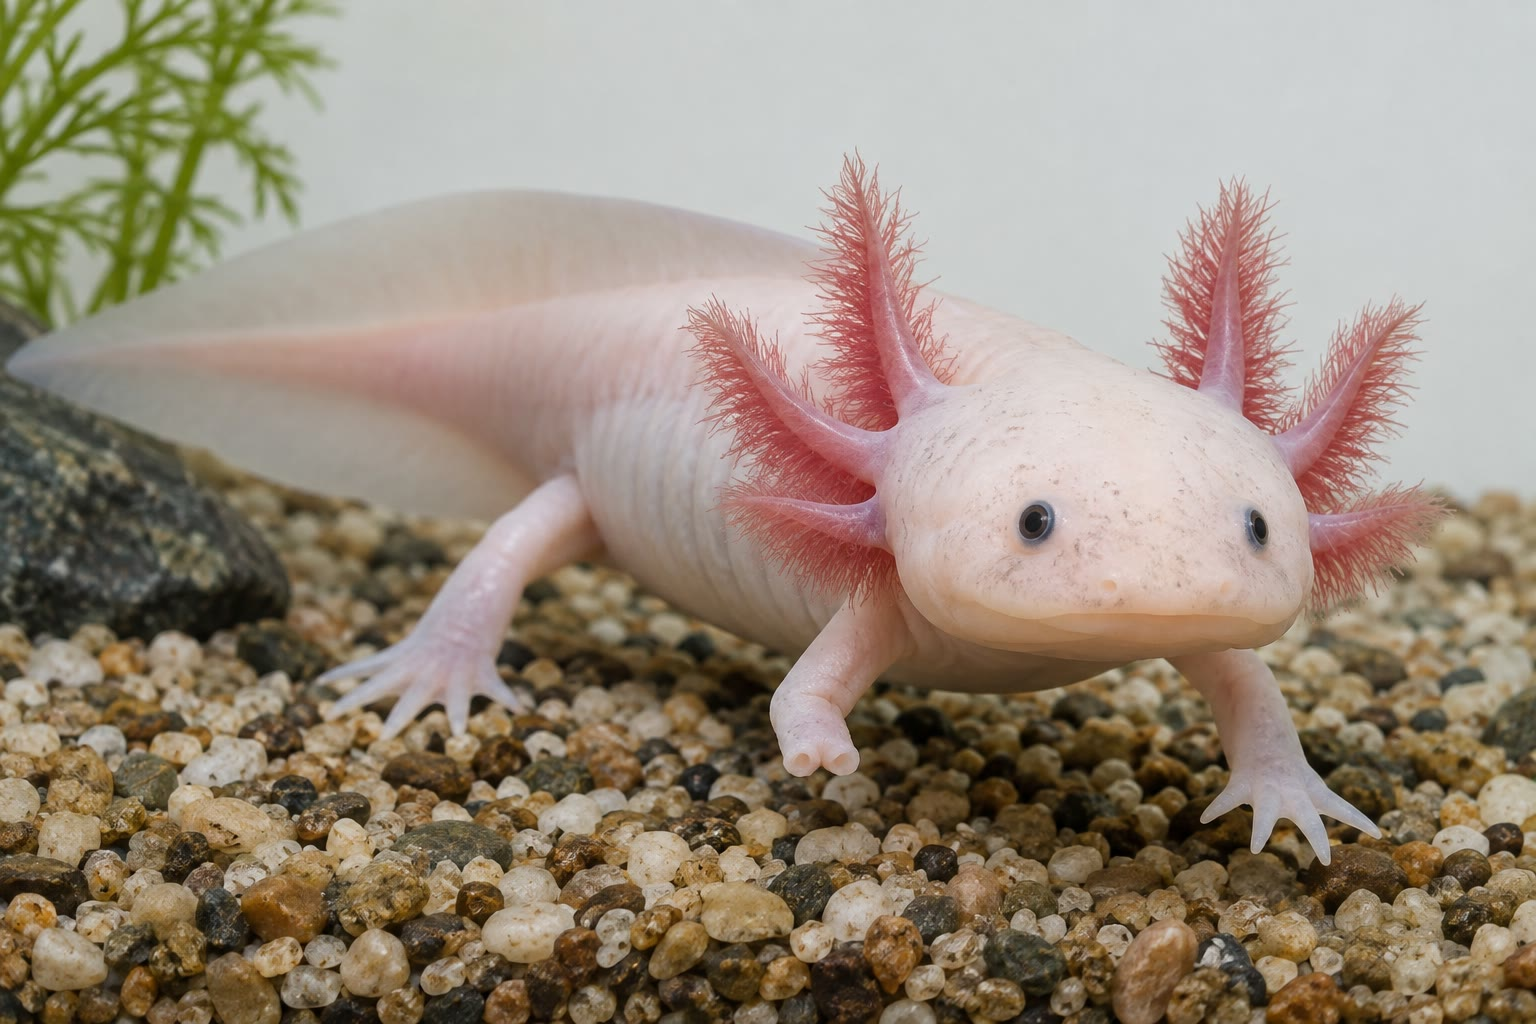
\includegraphics[width=0.46\linewidth]{images/book5/ai/b5-24-axolotl.jpg}\hspace{0.04\linewidth}
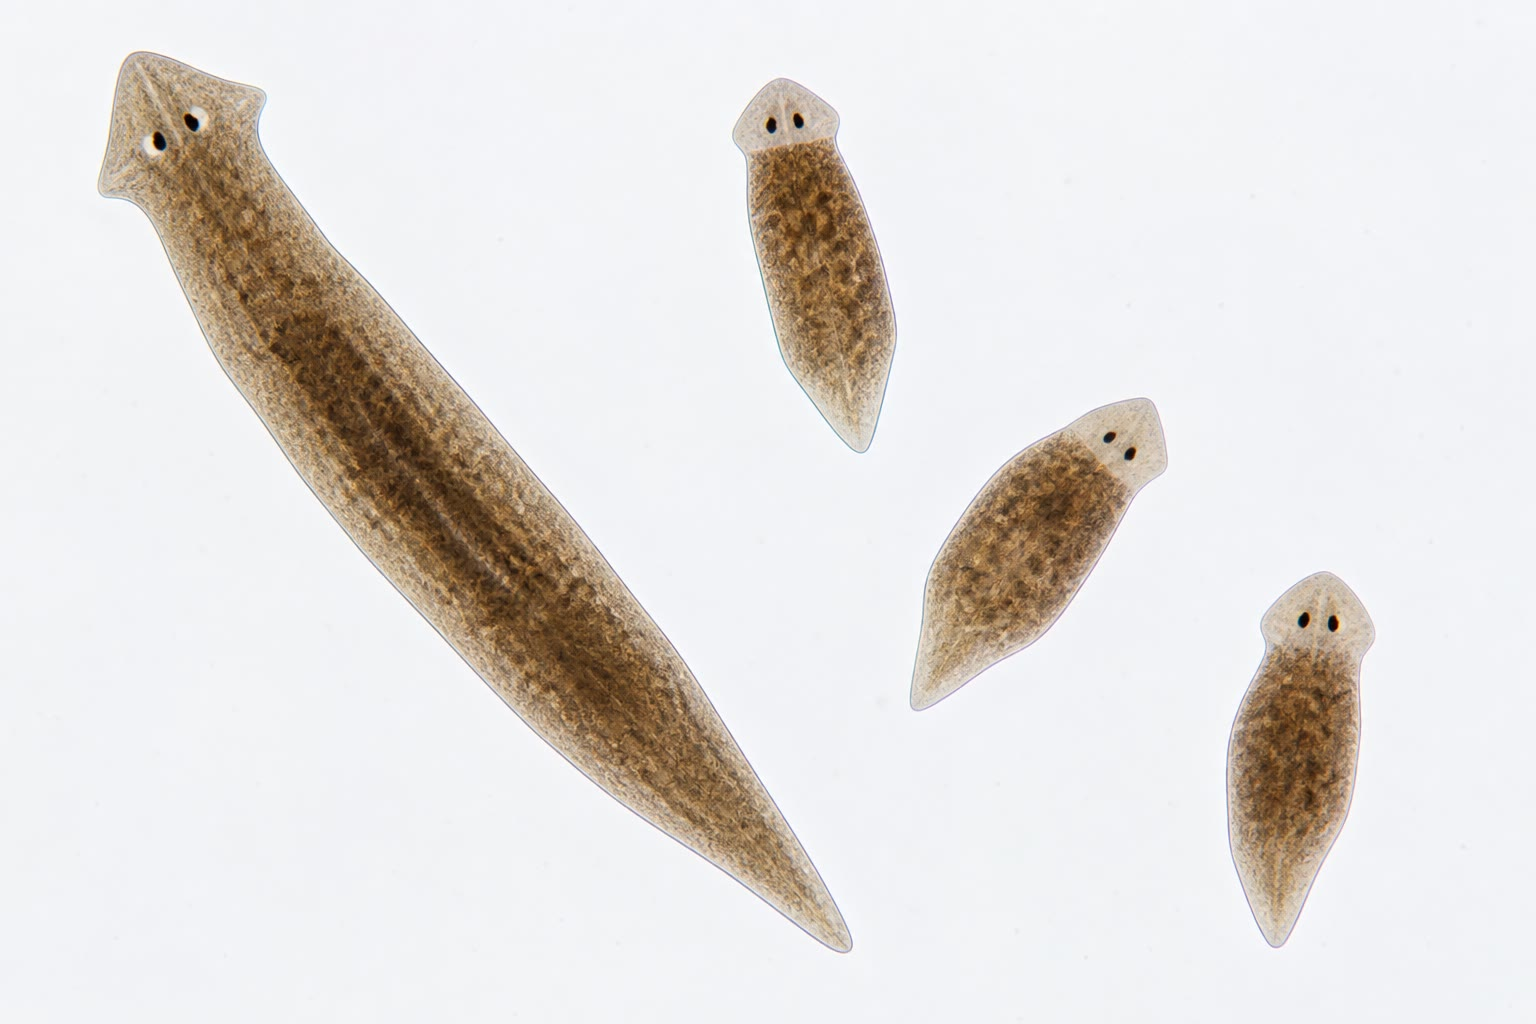
\includegraphics[width=0.46\linewidth]{images/book5/ai/b5-24-planarian-regeneration.jpg}

{\small يسارًا: أكسولوتل، يعيد إنماء طرف في شهرين من \omterm{def:b3:stem-cells:regeneration}{بلاستيما}
من خلايا مزالة التمايز ويقدر على ذلك طوال عمره. ويمينًا:
بلاناريا قُطعت قطعًا، وكل قطعة تعيد إنماء دودة كاملة من
نيوبلاستاتها في غضون أسبوعين.}
\end{omfigure}

\begin{proof}[شواهد]
قطع مورغان (1898) البلاناريا إلى 279 قطعة فوجد كل قطعة تعيد
إنماء دودة كاملة إلى حدّ نحو جزء من مئة من الجسم؛ وزرع ريدين
وزملاؤه (2011) نيوبلاستًا واحدًا في دودة مشععة تشعيعًا قاتلًا
فاستعادتها كلها --- خلية واحدة، وكل نسيج. وصنع كراغل وزملاؤه
(2009) أكسولوتلات وُسمت نسجها بالأخضر نسيجًا بعد نسيج
وطعّموها في مضائف غير موسومة: فبعد البتر، لم يعطِ العضل
الأخضر إلا عضلًا، ولا الغضروف الأخضر إلا غضروفًا ---
\omterm{def:b3:stem-cells:regeneration}{فالبلاستيما} ليست مجمعًا من خلايا كاملة القدرات بل مجموعة من
سلائف محصورة السلالة، كل واحدة مزالة التمايز إلى حدّ \omterm{def:b3:stem-cells:stem}{سليفة}
نسيجها هي لا أبعد. وبيّن سينغر (1952) أن طرف السمندر لا
يتجدد إلا إذا بلغ الجذمور عددٌ عتبي من الألياف العصبية، وأن
تحويل عصب إلى جرح في الخاصرة جعل طرفًا ينمو هناك.
\end{proof}

\section{حساب الشيخوخة}

\begin{theorem}[التيلوميرات وحدّ هايفليك]\label{thm:b3:stem-cells:hayflick}
\index{تيلومير}\index{حد هايفليك}\index{مشكلة تضاعف النهاية}\index{تيلوميراز}\index{شيخوخة تضاعفية}
ينتهي كل صبغي \emph{بتيلومير}، أي عدة كيلوأسس من التكرار
TTAGGG. ولأن بوليميراز DNA لا يقدر على إتمام آخر امتداد من
الطاق المتأخر (وهي \emph{\omterm{thm:b3:stem-cells:hayflick}{مشكلة تضاعف النهاية}})، يقصّر كل
انقسام كل تيلومير بمقدار $\Delta \approx$ \qtyrange{50}{100}{bp}.
وانطلاقًا من $L_{0} \approx \qty{10}{kb}$ وبإطلاق
\emph{\omterm{thm:b3:stem-cells:hayflick}{الشيخوخة التضاعفية}} --- وهي توقف دائم يفرضه p53 ---
حين يبلغ أقصر تيلومير $L_{\text{crit}} \approx \qty{4}{kb}$،
تقدر سلالة خلوية على الانقسام على الأكثر
\[
n_{\max} = \frac{L_{0} - L_{\text{crit}}}{\Delta} \approx \frac{6000}{50\text{--}100} \approx 60\text{--}120
\]
مرة: وهو \emph{\omterm{thm:b3:stem-cells:hayflick}{حد هايفليك}}، أي مضاعفات الجمهرة الخمسون
ونيّف التي تتمها الأرومات الليفية البشرية في الاستنبات قبل
أن تتوقف. والإنزيم \emph{\omterm{def:b3:cancer-biology:telomerase}{التيلوميراز}}، وهو ناسخ عكسي قالبه
RNA، يمدّ النهايات من جديد؛ وهو فعال في السلالة الجنسية،
وفي الخلايا الجذعية الجنينية وكثير من البالغة، وفي
\qty{90}{\%} من السرطانات، التي أفلتت من الحد بإعادة تشغيله.
\omterm{def:b3:stem-cells:stem}{والخلية الجذعية} التي تنقسم $d$ مرة في السنة مع تعويض
\omterm{def:b3:cancer-biology:telomerase}{التيلوميراز} نسبةً $f$ من الفقد لها
$n_{\max} = (L_{0} - L_{\text{crit}})/[(1 - f)\Delta]$
انقسامًا، وعمر $n_{\max}/d$ سنة: فعند $f = 0.7$، و$\Delta
= 60$، و$d = 1$، نحو 330 سنة \omterm{def:b3:stem-cells:stem}{لخلية جذعية} مكوِّنة للدم --- غير
أن سلائفها، \omterm{def:b3:cancer-biology:telomerase}{والتيلوميراز} مطفأ وعشرون انقسامًا إلى الكرية
الحمراء، تنفق خُمس احتياطيها في كل سلالة، ولذلك تكون
تيلوميرات كريات دم المسنين أقصر من تيلوميرات الشباب، بنحو
\qty{30}{bp} في السنة.
\end{theorem}
\begin{proof}
الفقد في كل انقسام طول ثابت، فيهبط طول التيلومير هبوطًا
خطيًا مع رقم الانقسام، $L_{n} = L_{0} - n\Delta$، ويبلغ
$L_{\text{crit}}$ عند $n = (L_{0} - L_{\text{crit}})/\Delta$؛ ومع
التعويض الجزئي يكون الفقد الصافي في الانقسام $(1 - f)\Delta$.
وبيّن هايفليك ومورهيد (1961) أن الأرومات الليفية البشرية
السوية تتوقف بعد نحو خمسين مضاعفة مهما تكن ظروف الاستنبات،
وأن الخلايا المجمَّدة بعد عشرين مضاعفة والمذابة لا تتم إلا
الثلاثين الباقية --- فهي تعدّ الانقسامات لا الزمن --- وأن
الحد أدنى في خلايا متبرعين مسنين. وقاس هارلي وفاتشر
وغرايدر (1990) تقصّر التيلوميرات مع المضاعفات في الاستنبات
ومع عمر المتبرع؛ ووضع بودنار وزملاؤه (1998) \omterm{def:b3:cancer-biology:telomerase}{التيلوميراز} في
خلايا سوية فانقسمت بعد الحد إلى ما لا نهاية من غير أن تصير
سرطانية، وهو ما أثبت التيلومير ساعةً.
\end{proof}

\begin{omfigure}
\begin{tikzpicture}
\begin{axis}[
  width=0.62\linewidth, height=5.4cm,
  axis x line=bottom, axis y line=left,
  xmin=0, xmax=120, ymin=0, ymax=11,
  xlabel={مضاعفات الجمهرة}, ylabel={طول التيلومير (kb)},
  xlabel style={font=\small, at={(axis description cs:0.5,-0.12)}, anchor=north}, ylabel style={font=\small},
  tick label style={font=\small}, xtick={0,30,60,90,120}, ytick={4,7,10},
  clip=false,
]
\addplot[very thick, omDef, domain=0:60, samples=2] {10-0.1*x};
\addplot[very thick, omThm, domain=0:120, samples=2] {10-0.05*x};
\addplot[very thick, omMeth!70!black, domain=0:120, samples=2] {10-0.015*x};
\draw[dashed, gray] (axis cs:0,4) -- (axis cs:120,4); \node[font=\scriptsize, gray, anchor=north west] at (axis cs:2,3.9) {شيخوخة عند $L_{\text{crit}} = \qty{4}{kb}$};
\node[font=\scriptsize, omDef, anchor=south west] at (axis cs:63,4.3) {$\Delta = \qty{100}{bp}$: 60 مضاعفة};
\node[font=\scriptsize, omThm, anchor=west] at (axis cs:70,8.0) {$\Delta = \qty{50}{bp}$: 120};
\node[font=\scriptsize, omMeth!70!black, anchor=south west, align=left] at (axis cs:78,9.3) {تيلوميراز يعوّض\\\qty{70}{\%}: 400};
\fill[omDef] (axis cs:60,4) circle (2pt); \fill[omThm] (axis cs:120,4) circle (2pt);
\end{axis}
\end{tikzpicture}

{\small التيلوميرات عدّادًا للانقسامات. فقدٌ ثابت في كل
انقسام يعطي خطًا مستقيمًا؛ وحيث يعبر الطولَ الحرج تتوقف
السلالة. \omterm{def:b3:cancer-biology:telomerase}{والتيلوميراز} يفلطح الميل، وإذا كان فعالًا تمامًا
ألغى الحد --- في السلالة الجنسية، وفي السرطانات.}
\end{omfigure}

\begin{proposition}[قانون غومبرتز]\label{prop:b3:stem-cells:gompertz}
\index{قانون غومبرتز}\index{معدل الوفاة}\index{معالم الشيخوخة}\index{خلية هرِمة}
فوق الثلاثين تقريبًا يتضاعف معدل وفاة الإنسان $\mu(t)$ ---
أي احتمال الموت في السنة التالية --- كل ثماني سنوات: $\mu(t) =
\mu_{0}\,\mathrm{e}^{\gamma(t - t_{0})}$ عند $\gamma = \ln 2/8 \approx
\qty{0.087}{yr^{-1}}$ (غومبرتز، 1825). ويكون البقاء إلى العمر $t$ عندئذ
\[
S(t) = \exp\!\Bigl[-\frac{\mu_{0}}{\gamma}\bigl(\mathrm{e}^{\gamma(t - t_{0})} - 1\bigr)\Bigr],
\]
وهو منحنٍ مستوٍ عقودًا ثم يهبط هبوطًا حادًّا، بعمر وسيط
$t_{1/2} = t_{0} + \gamma^{-1}\ln(1 + \gamma\ln 2/\mu_{0})$:
فعند $\mu_{0} = 10^{-3}$ في السنة عند الثلاثين، نحو $30 + 47 = 77$ سنة.
والقانون نفسه، بثوابت مختلفة، يصح للفئران (وزمن مضاعفتها
ثلاثة أشهر)، وللكلاب، وللذباب، وللديدان: فالشيخوخة ارتفاع
أسّي في القابلية للأذى، لا ساعة تقف. والبيولوجيا وراء الأس
مجموعة من \emph{المعالم} المتفاعلة: أذى DNA المتراكم
والانجراف اللاجيني، وتآكل التيلوميرات، وفقد استتباب
البروتين، وتدهور المتقدرات، واستنفاد مجامع الخلايا الجذعية،
وتراكم \emph{الخلايا الهرِمة} التي لم تعد تنقسم لكنها تفرز
إشارات التهابية، \omterm{def:b3:innate-immunity:inflammation}{والالتهاب} المزمن؛ وفي الفئران، يطيل تنقيةُ
الخلايا الهرِمة أو تقييدُ السعرات العمرَ، وفي الديدان تضاعفه
طفرة واحدة في السبيل الشبيه \omterm{def:b3:endocrinology:glucose}{بالأنسولين}. وأما هل يمكن خفض
الأس في البشر، بدل الثابت $\mu_{0}$
الذي خفضه الطب عشرة أضعاف في قرن، فهو السؤال المفتوح.
\end{proposition}
\begin{proof}
إذا كان $\mu$ هو الخطر، كان $\mathrm{d}S/\mathrm{d}t = -\mu(t)S$، فيكون $\ln S =
-\int_{t_{0}}^{t}\mu = -(\mu_{0}/\gamma)(\mathrm{e}^{\gamma(t-t_{0})} -
1)$. وبوضع $S = 1/2$: $\mathrm{e}^{\gamma(t-t_{0})} = 1 + \gamma\ln 2/
\mu_{0}$، ومنه الوسيط؛ وعند $\gamma = 0.087$ و$\mu_{0} =
10^{-3}$، $\ln(1 + 60) = 4.1$، و$t - t_{0} = 47$. والقانون التجريبي
مطابقة غومبرتز لجداول الحياة الإنكليزية؛ وأما أنه يصف أنواعًا
كثيرة بصورة مشتركة وثوابت خاصة بكل نوع فمسلَّم به هنا خلاصةً
لقرن من علم السكان.
\end{proof}

\begin{omfigure}
\begin{tikzpicture}
\begin{semilogyaxis}[
  width=0.5\linewidth, height=5.2cm,
  axis x line=bottom, axis y line=left,
  xmin=20, xmax=100, ymin=0.0003, ymax=1,
  xlabel={العمر (بالسنوات)}, ylabel={معدل الوفاة في السنة},
  xlabel style={font=\small, at={(axis description cs:0.5,-0.12)}, anchor=north}, ylabel style={font=\small},
  tick label style={font=\small}, xtick={30,50,70,90}, ytick={0.001,0.01,0.1,1}, yticklabels={0.001,0.01,0.1,1},
  clip=false,
]
\addplot[very thick, omDef, domain=30:100, samples=2] {0.001*exp(0.0866*(x-30))};
\node[font=\scriptsize, omDef, anchor=north west, align=left] at (axis cs:32,0.3) {$\mu = \mu_{0}\,\mathrm{e}^{\gamma(t-30)}$\\يتضاعف كل 8 سنوات};
\end{semilogyaxis}
\begin{axis}[
  at={(0.55\linewidth,0)}, anchor=south west,
  width=0.43\linewidth, height=5.2cm,
  axis x line=bottom, axis y line=left,
  xmin=20, xmax=110, ymin=0, ymax=1.05,
  xlabel={العمر (بالسنوات)}, ylabel={نسبة الباقين},
  xlabel style={font=\small, at={(axis description cs:0.5,-0.12)}, anchor=north}, ylabel style={font=\small},
  tick label style={font=\small}, xtick={30,50,77,100}, ytick={0.5,1},
  clip=false,
]
\addplot[very thick, omThm, domain=30:110, samples=80] {exp(-(0.001/0.0866)*(exp(0.0866*(x-30))-1))};
\draw[dashed, gray] (axis cs:77,0) -- (axis cs:77,0.5) -- (axis cs:20,0.5);
\node[font=\scriptsize, omThm, anchor=north east, align=right] at (axis cs:75,0.45) {الوسيط\\77 سنة};
\end{axis}
\end{tikzpicture}

{\small \omterm{prop:b3:stem-cells:gompertz}{قانون غومبرتز}. يسارًا: على محور لوغاريتمي يكون \omterm{prop:b3:stem-cells:gompertz}{معدل
الوفاة} خطًا مستقيمًا من الثلاثين فصاعدًا. ويمينًا: منحنى
البقاء الذي يتبع --- هضبة، ثم جرف، والوسيط حيث يبلغ تكامل
الخطر $\ln 2$.}
\end{omfigure}

\begin{remark}[التجدد وثمنه]\label{rem:b3:stem-cells:remark}
الجسم الذي يجدد نفسه لا بد أن يحتفظ بخلايا تقدر على الانقسام
بلا نهاية، والخلايا التي تقدر على الانقسام بلا نهاية هي مادة
\omterm{def:b3:cancer-biology:hallmarks}{السرطان}؛ والجسم الذي يحترس من \omterm{def:b3:cancer-biology:hallmarks}{السرطان} بعدّ الانقسامات وفرض
الشيخوخة لا بد أن ينقصه، مع الوقت، ما يقدر على الانقسام.
وتراتب الخلايا الجذعية حل --- خلايا قليلة بطيئة محميّة في
حاضنات، وخلايا كثيرة سريعة تموت قريبًا --- وحدّ هايفليك حل
آخر، وأسّي غومبرتز مجموع كلفتيهما. والسمندر يدفع دفعًا آخر:
فهو يحتمل خلايا تزيل تمايزها ويعيد إنماء رجل، وهو بارد الدم
بطيء نادرًا ما يعيش طويلًا بما يكفي لدفع فاتورة \omterm{def:b3:cancer-biology:hallmarks}{السرطان}.
فالخلايا التي وُلدت بها ليست، في معظمها، الخلايا التي عندك؛
وأما التي صنعت البدائل فهي التي عليك أن تحفظها.
\end{remark}

\section{تمارين}

\begin{exercise}[$\star$]\label{exo:b3:stem-cells:1}
عرّف \omterm{def:b3:stem-cells:stem}{التجدد الذاتي}، والقدرة، \omterm{def:b3:stem-cells:stem}{والحاضنة}، \omterm{def:b3:stem-cells:stem}{وخلية العبور
المضخِّمة}، واذكر مثالًا على كل منها في الأمعاء.
\end{exercise}

\begin{exercise}[$\star$]\label{exo:b3:stem-cells:2}
ماذا أظهرت مقايسة مستعمرات الطحال، وأي خاصية من خصائص \omterm{def:b3:stem-cells:stem}{الخلية
الجذعية} اقتضت فأرًا ثانيًا لبيانها؟
\end{exercise}

\begin{exercise}[$\star$]\label{exo:b3:stem-cells:3}
سمّ عوامل يامانكا الأربعة واشرح لماذا تستغرق \omterm{def:b3:stem-cells:pluripotency}{إعادة البرمجة}
أسابيع وتنجح في جزء من ألف من الخلايا.
\end{exercise}

\begin{exercise}[$\star$]\label{exo:b3:stem-cells:4}
قابل بين طريقي البلاناريا والسمندر إلى \omterm{def:b3:stem-cells:regeneration}{التجدد}، وقل ماذا
أظهرت تجارب التطعيم عند كراغل عن \omterm{def:b3:stem-cells:regeneration}{البلاستيما}.
\end{exercise}

\begin{exercise}[$\star\star$]\label{exo:b3:stem-cells:5}
تبدأ التيلوميرات عند \qty{11}{kb}، والشيخوخة عند \qty{5}{kb}،
والفقد \qty{75}{bp} في الانقسام. فما حدّ هايفليك؟ وخلايا من
متبرع عمره 70 سنة عندها \qty{8}{kb}: فكم مضاعفة تبقى؟ وإذا
عوّض \omterm{def:b3:cancer-biology:telomerase}{التيلوميراز} \qty{60}{\%} من الفقد، فما الحد؟
\end{exercise}

\begin{exercise}[$\star\star$]\label{exo:b3:stem-cells:6}
خبيئة فيها 14 \omterm{def:b3:stem-cells:stem}{خلية جذعية} تنقسم مرة في اليوم، تغذي خلايا عبور
تنقسم 4 مرات أخرى، والخبيئة تزوّد زغابتها بعدد \num{300} خلية في
اليوم. تحقق من الحساب: كم انقسامًا جذعيًا في اليوم ينتج بنات
متمايزات، وكم يعادل ذلك من انقسامات خلايا جذعية؟
\end{exercise}

\begin{exercise}[$\star\star$]\label{exo:b3:stem-cells:7}
يصنع الجسم $2\times 10^{11}$ كرية حمراء في اليوم، كل واحدة
ناتج نحو 20 انقسامًا من \omterm{def:b3:stem-cells:stem}{خلية جذعية}. فكم انقسامًا جذعيًا في
اليوم يقتضي ذلك، وبوجود \num{10000} \omterm{def:b3:stem-cells:stem}{خلية جذعية}، كم مرة تنقسم
كل واحدة؟ وقارن ذلك بالمرصود ``نحو مرة في السنة'' واشرح
التفاوت.
\end{exercise}

\begin{exercise}[$\star\star$]\label{exo:b3:stem-cells:8}
عند $\gamma = \qty{0.087}{yr^{-1}}$ و$\mu_{0} = 10^{-3}$ عند
الثلاثين، احسب \omterm{prop:b3:stem-cells:gompertz}{معدل الوفاة} عند 50 و70 و90، والبقاء إلى 70
و90، والعمر الوسيط. وماذا يفعل تنصيف $\mu_{0}$ بالوسيط؟ وماذا
يفعل تنصيف $\gamma$؟
\end{exercise}

\begin{exercise}[$\star\star$]\label{exo:b3:stem-cells:9}
يُزال ثلثا كبد جرذ. والخلايا الكبدية الباقية، وكلها تنقسم،
تستعيد الكتلة في عشرة أيام. فكم انقسامًا تحتاج كل واحدة؟
ولماذا يُسمّى ذلك نموًا تعويضيًا لا تجددًا، وما الذي
\emph{لا} يعيد الكبد بناءه؟
\end{exercise}

\begin{exercise}[$\star\star\star$]\label{exo:b3:stem-cells:10}
\omterm{prop:b3:stem-cells:crypt}{الانجراف المحايد}: $N$ \omterm{def:b3:stem-cells:stem}{خلية جذعية} في \omterm{def:b3:stem-cells:stem}{حاضنة} تنقسم انقسامًا
متناظرًا؛ وفي كل حدث تنقسم خلية وتضيع أخرى عشوائيًا، فيؤدي
عدد نسيلة معينة مشيًا عشوائيًا بين $0$ و$N$. احتجّ لأن احتمال
أن تستولي نسيلة من $k$ خلية على \omterm{def:b3:stem-cells:stem}{الحاضنة} في النهاية هو
$k/N$، ولأن نسيلة من خلية واحدة عند $N = 14$ حظها $1/14$.
وبماذا يتنبأ ذلك عن مصير \omterm{def:b3:stem-cells:stem}{خلية جذعية} تحمل طفرة محايدة جديدة؟
\end{exercise}

\begin{exercise}[$\star\star\star$]\label{exo:b3:stem-cells:11}
طفرة تعطي نسيلة جذعية أفضلية \qty{10}{\%} في تنافس
\cref{exo:b3:stem-cells:10}. اشرح نوعيًا لماذا يرتفع احتمال
استيلائها فوق $k/N$ كثيرًا، ولماذا تهيمن بضع نسائل أكثر
فأكثر على خبيئات المسنين ونقيهم (تكوين الدم النسيلي)، ولماذا
تكون تلك خطوة أولى نحو \omterm{def:b3:cancer-biology:hallmarks}{السرطان} من غير أن تكون سرطانًا.
\end{exercise}

\begin{exercise}[$\star\star\star$]\label{exo:b3:stem-cells:12}
افترض أن أس غومبرتز $\gamma$ يعكس معدل تراكم الأذى وأن
الثابت $\mu_{0}$ يعكس البيئة. وقد خفض الطب $\mu_{0}$ عشرة
أضعاف منذ 1900 من غير أن يغيّر $\gamma$. احسب المكسب في العمر
الوسيط من ذلك الخفض العشري، والمكسب الإضافي من خفض عشري آخر؛
واشرح لماذا تتناقص العوائد، وماذا كان سيفعل خفض $\gamma$
بمقدار \qty{20}{\%} بدل ذلك.
\end{exercise}

\section{مسألة: الخلايا التي وُلدت بها}

\begin{problem}[{مسألة نهاية الأسبوع --- تجدد جسد بالأرقام:
تراتب الدم وما يطلبه من خلاياه الجذعية، وانجراف الخبيئة،
وساعة التيلومير وكيف ينفقها التيلوميراز والسلائف، ومنحنى
غومبرتز للجمهرة، والمقايضات التي يقبلها حيوان متجدد، وتُختم
بعدّة هايفليك، وباحتياطي الخلية الجذعية على مدى العمر،
وبالعمر الوسيط}]
\label{pb:b3:stem-cells:1}
المعطيات: كريات حمر $2.5\times 10^{11}$ في اليوم، ومحببات
$10^{11}$ في اليوم؛ و$20$ انقسامًا من \omterm{def:b3:stem-cells:stem}{الخلية الجذعية} إلى
الخلية الناضجة؛ و\num{10000} \omterm{def:b3:stem-cells:stem}{خلية جذعية} مكوِّنة للدم.
والتيلوميرات: $L_{0} = \qty{10}{kb}$،
و$L_{\text{crit}} = \qty{4}{kb}$، و$\Delta = \qty{60}{bp}$ في الانقسام؛
\omterm{def:b3:cancer-biology:telomerase}{والتيلوميراز} في الخلايا الجذعية يعوّض $f = 0.7$؛ ولا شيء في
السلائف. والخبيئة: $N = 14$ \omterm{def:b3:stem-cells:stem}{خلية جذعية}، وانقسام واحد في
اليوم. وغومبرتز: $\mu_{0} =
10^{-3}$ في السنة عند العمر 30، و$\gamma = \qty{0.087}{yr^{-1}}$.
وطرف الأكسولوتل: \qty{40}{mm} يُعاد إنماؤها في \qty{60}{d}؛
\omterm{def:b3:stem-cells:regeneration}{والبلاستيما} $10^{5}$ خلية تنمو إلى $10^{8}$.

\medskip
\noindent\textbf{الجزء الأول --- الدم.}
\begin{enumerate}
  \item الخلايا المنتَجة في اليوم إجمالًا، وفي الثانية.
  \item كل خلية ناضجة نهاية $20$ انقسامًا: فكم خلية تنتج من
        بنت ملتزمة واحدة \omterm{def:b3:stem-cells:stem}{لخلية جذعية}؟ وكم بنتًا ملتزمة في
        اليوم تلزم؟
  \item مع \num{10000} \omterm{def:b3:stem-cells:stem}{خلية جذعية}، كم انقسامًا متمايزًا لكل
        \omterm{def:b3:stem-cells:stem}{خلية جذعية} في اليوم يقتضي ذلك؟ وفي السنة؟
  \item الانقسام الجذعي المقيس نحو مرة في السنة. وفّق بين
        الأمرين: ما الذي يجب أن تفعله السلائف مما افترض حساب
        السؤال~3 أن الخلايا الجذعية تفعله؟
  \item لا \omterm{def:b3:cancer-biology:telomerase}{تيلوميراز} في السلائف. فانطلاقًا من \qty{10}{kb}، أي
        طول تيلومير تبلغه \omterm{def:b3:stem-cells:stem}{سليفة} كرية حمراء بعد انقساماتها
        $20$؟ وهل يهم أنه فوق $L_{\text{crit}}$؟
  \item \omterm{def:b3:stem-cells:stem}{خلية جذعية} تنقسم مرة في السنة عند $f = 0.7$: الفقد
        الصافي في الانقسام، والانقسامات حتى الشيخوخة، والسنون.
        علّق.
\end{enumerate}

\medskip
\noindent\textbf{الجزء الثاني --- الخبيئة.}
\begin{enumerate}[resume]
  \item الانقسامات في الخبيئة في اليوم عند طبقة الخلايا
        الجذعية؛ وإذا استبدل نصف الأحداث \omterm{def:b3:stem-cells:stem}{خلية جذعية} ضائعة
        وغذّى نصفها منطقة العبور، فكم خلية ملتزمة في اليوم،
        وكم خلية زغابية بعد $4$ انقسامات عبور؟
  \item احتمال استيلاء نسيلة من خلية واحدة هو $1/N$. والزمن
        المتوقع حتى أحادية النسيلة من رتبة $N^{2}$ حدث انقسام
        لكل خلية؛ قدّره بالأيام وقارنه بمشاهدات الكونفيتّي
        (أشهر).
  \item تكتسب \omterm{def:b3:stem-cells:stem}{خلية جذعية} طفرة. فما احتمال تثبّتها في خبيئتها
        في النهاية؟ وفي كم خبيئة من خبيئات القولون البالغة
        $10^{7}$ تتثبت طفرة تنشأ مرة في كل خبيئة؟
  \item لماذا يحمي انجراف الخبيئة من \omterm{def:b3:cancer-biology:hallmarks}{السرطان} أكثر مما يحمي
        نسيجٌ تنقسم فيه كل \omterm{def:b3:stem-cells:stem}{خلية جذعية} انقسامًا لامتناظرًا مدى
        الحياة؟
  \item بعد أن يقتل التشعيع الخلايا الجذعية، ترتدّ خلايا
        العبور وتملأ \omterm{def:b3:stem-cells:stem}{الحاضنة}. فبماذا يدل ذلك على أين تسكن
        الجذعية؟
  \item ارسم تجربة \omterm{met:b3:stem-cells:tracing}{تتبع السلالة} التي تميّز الانجراف المتناظر
        من \omterm{def:b3:stem-cells:stem}{الانقسام اللامتناظر}، والنتيجتين.
\end{enumerate}

\medskip
\noindent\textbf{الجزء الثالث --- الساعة.}
\begin{enumerate}[resume]
  \item حدّ هايفليك لسلالة جسدية بلا \omterm{def:b3:cancer-biology:telomerase}{تيلوميراز}.
  \item يُجمَّد استنبات أرومات ليفية بعد $25$ مضاعفة ويُذاب
        بعد عقد: فكم مضاعفة تبقى؟ وبماذا يدل ذلك على ما
        تعدّه الخلية؟
  \item تقصر تيلوميرات الكريات البيض \qty{30}{bp} في السنة عند
        البالغين. فانطلاقًا من \qty{8}{kb} عند العشرين، متى
        تبلغ $L_{\text{crit}}$؟ قارن ذلك بطول العمر وعلّق.
  \item \omterm{def:b3:cancer-biology:telomerase}{التيلوميراز} المضاف إلى أرومات ليفية سوية يجعلها تتجاوز
        الحد من غير أن تصير سرطانية. \omterm{def:b3:cancer-biology:telomerase}{والتيلوميراز} فعال في
        \qty{90}{\%} من السرطانات. وفّق بين العبارتين.
  \item احسب معدل وفاة غومبرتز عند 40 و60 و80 و100، والبقاء
        إلى كل منها.
  \item العمر الوسيط؛ والعمر الذي يبقى عنده \qty{10}{\%}.
\end{enumerate}

\medskip
\noindent\textbf{الجزء الرابع --- إعادة الإنماء.}
\begin{enumerate}[resume]
  \item الأكسولوتل: متوسط معدل إعادة الإنماء بالميليمتر في
        اليوم؛ والمضاعفات اللازمة لتنمو \omterm{def:b3:stem-cells:regeneration}{البلاستيما} من $10^{5}$
        إلى $10^{8}$ خلية، ومتوسط زمن المضاعفة على مدى 60 يومًا.
  \item إذا انقسمت الخلايا المزالة التمايز كخلايا \omterm{def:b3:stem-cells:regeneration}{البلاستيما}
        طوال العمر وحمل الانقسام احتمال $10^{-9}$ لكل خلية
        لطفرة مسرطِنة، فكم طفرة من هذا القبيل تنشأ في \omterm{def:b3:stem-cells:regeneration}{تجدد}
        واحد؟ ولماذا لا يكاد الأكسولوتل مع ذلك يُصاب \omterm{def:b3:cancer-biology:hallmarks}{بالسرطان}،
        ولماذا قد لا ينجو ثديي بذلك؟
  \item نزع عصب الجذمور يوقف \omterm{def:b3:stem-cells:regeneration}{التجدد}. اقترح تجربة تبيّن أن
        العصب يوفر عاملًا قابلًا للانتشار، وهوية ممكنة واحدة
        لذلك العامل.
  \item قطعة ذنب من بلاناريا تُنمي ذنبًا ثانيًا بدل رأس حين
        يُخفَض مثبط Wnt. اشرح ذلك بتدرج وبذاكرة القطعة
        الموضعية.
  \item كبد الإنسان بعد استئصال الثلثين: ما نسبة الخلايا
        الكبدية التي يجب أن تنقسم مرة، ومرتين، لاستعادة
        الكتلة؟ ولماذا تكون النتيجة كبدًا عاملًا لكن بالشكل
        الخطأ؟
  \item لماذا يكون لجسد يتجدد كالأكسولوتل منحنى غومبرتز
        مختلف، وفي أي اتجاه؟
  \item لخّص: عدّة هايفليك (السؤال~13)، وانقسامات \omterm{def:b3:stem-cells:stem}{خلية جذعية}
        معانة \omterm{def:b3:cancer-biology:telomerase}{بالتيلوميراز} وسنوها (السؤال~6)، والعمر الوسيط
        (السؤال~18).
\end{enumerate}
\end{problem}
